\chapter{Implications for model evaluation: an informed comparison of cloud and
radiative properties in CMIP5 models}\label{cmip5_chapter}
With the uncertainty analysis in Chapter \ref{misr_chapter} and the identification in Chapters \ref{subgrid1_chapter} and \ref{subgrid2_chapter} of potential ambiguities in results due to treatments of unresolved clouds and precipitation in simulating satellite diagnostics from COSP, the question remains: what conclusions can be robustly determined by comparing clouds retrieved from space with simulated views of clouds from space? In other words, which differences identified between modeled and observed cloud statistics can be attributed to model biases, as opposed to limitations or errors in the current framework? This question is explored in this chapter in the context of an inter-comparison of cloud and radiative flux statistics in a selection of five different global climate models, which all participated in CMIP5/CFMIP2.

\section{Models and observations}
Five models are compared in this study using COSP output generated from the inline implementation of COSP within each model: the Geophysics Fluid Dynamics Laboratory (GFDL) AM3 \citep{donner_et_al_2011}, the National Center for Atmospheric Research (NCAR) CAM4 \citep{neale_et_al_2010a} and CAM5 \citep{neale_et_al_2010b}, the Canadian Centre for Climate Modeling and Analysis (CCCma) CanAM4 \citep{von_salzen_et_al_2012}, and the UK Met Office Hadley Center (MOHC) HadGEM2 \citep{martin_et_al_2011}. These models are the atmosphere-only components of the fully-coupled earth system models produced by each respective institution. The simulations presented here were run in ``AMIP'' configuration [citations], in which the model is forced by observed sea-surface-temperatures and run without an interactive ocean component.

The analysis presented here compares simulated views of clouds from COSP between models and against satellite retrievals, and connects identified biases in cloud statistics with biases in cloud radiative effects. Each of the models evaluated here have included COSP into their source code, and COSP outputs were generated by running COSP inline with the model for the length of the simulation time. 

Each of the participating modeling centers have provided both the MISR and ISCCP-simulated cloud top height (or pressure) and optical depth (CTH-OD or CTP-OD) joint histogram outputs from COSP. These outputs are evaluated against the corresponding CTH-OD and CTP-OD datasets produced by the MISR and ISCCP science teams, available as monthly-mean gridded products from the CFMIP archive\footnote{\tt http://climserv.ipsl.polytechnique.fr/fr/cfmip-observations.html}. These datasets are briefly summarized here, and a more comprehensive description can be found in \cite{marchand_et_al_2010}.

[this whole section needs to be re-written. Focus on the utility of the CTH-OD datasets in jointly characterizing both the shortwave CRE (through optical depth) and the longwave CRE (through cloud top height).]

ISCCP collects data from visible and infrared imagers on a number of both geostationary and polar-orbiting satellite and combines these measurements into a single cloud product. Among the retrieved cloud properties are histograms of cloud top pressure ($p_c$) and cloud optical depth ($\tau$). To calculate the frequency of clouds with cloud top pressures at low altitudes (low-topped clouds), the CTP-OD joint histogram is summed over all bins with $p_c > 680$ hPa and $\tau > 0.3$. The restriction of $\tau > 0.3$ in the model calculations is necessary for consistency among the different observations and model diagnostics because this is approximately the limit of the instrument sensitivity for ISCCP and MISR \citep{marchand_et_al_2010}. Recent studies have pointed to considerable observational uncertainty in cloud amount at the low end of the optical depth range and have suggested a somewhat higher threshold to restrict the population of clouds for comparison \citep[e.g.,][]{pincus_et_al_2012, zhao_and_digirolamo_2006}. The analysis here will evaluate errors using thresholds of both $\tau > 0.3$ and $\tau > 1.3$, but the smaller threshold will be used by default to obtain a more comprehensive sample of cloud types (e.g., broken clouds). The large differences between models and observations using the lower threshold in regions dominated by broken boundary layer clouds will highlight the large observational uncertainty surrounding these cloud types. Mid-topped clouds are similarly defined as those with $440 < p_c < 680$ hPa, and high-topped clouds are defined as those with $p_c < 440$ hPa.

As discussed in Chapter \ref{misr_chapter}, the MISR instrument has a unique arrangement of nine different cameras, each pointed at a different viewing angle along the satellite track. The successive imaging of cloud scenes from different angles allows MISR to use a stereo imaging technique to retrieve cloud top heights ($z_c$) as opposed to the cloud brightness temperature technique used by ISCCP and other single-camera radiometer-based retrievals \citep{moroney_et_al_2002, muller_et_al_2002}. One of the consequences of this is that MISR sees through optically thin, high-level clouds and retrieves the cloud otp height of the underlying cloud layer in cases of multi-layered cloud scenes involving optically thin high-level cloud over an optically thicker cloud layer \citep{marchand_et_al_2010}. Thus, low-topped cloud amounts from MISR tend to be higher than those from ISCCP, while mid and high-topped cloud amounts tend to be lower. For MISR, low-topped clouds are defined as those with $z_c < 3$ km, mid-topped clouds are defined as those with $3 < z_c < 7$ km, and high-topped clouds are defined as those with $z_c > 7$ km.

[Discussion of different optical depth categories here.]

Radiative fluxes are evaluated against the Clouds and the Earths Radiant Energy Balanced and Filled dataset \citep[CERES-EBAF Version 2.6;][]{loeb_et_al_2009}. This dataset was developed specifically for climate model evaluation. The shortwave and longwave fluxes in this dataset have been adjusted within the observational uncertainty to obtain a net top of atmosphere (TOA) energy balance that ismore consistent with estimates of global heat storage. The CERES-EBAF dataset covers the time period from the year 2000 to present, and is available directly from the CERES team\footnote{\tt https://ceres-tool.larc.nasa.gov/ord-tool/srbavg}, or from CFMIP in gridded, monthly averaged form\footnote{\tt <url to CFMIP source?>}.

The instantaneous effect of clouds on the TOA radiation budget can be quantified by calculating the difference between the all-sky and clear-sky fluxes \citep[e.g.,][]{ellis_and_vonderhaar_1976, ramanathan_1987, ramanathan_et_al_1989}. In this context, clear-sky means non-cloudy, so aerosol effects are implicitely contained in the clear-sky fluxes. The resulting quantity is commonly referred to as the cloud radiative forcing or CRF. This language is somewhat misleading, however, as this quantity is not strictly a forcing, but rather a measure of the effect of clouds on the instantaneous TOA fluxes \citep{stephens_2005}. A more appropriate term for this quantity is the cloud radiative effect, or simply the CRE, and it will be referred as such here. The CRE can be calculated separately for the shortwave and longwave fluxes, and model biases will be evaluated separately in each of these broad spectral bands here.

Because MISR cloud optical depths are not computed over land or ice, MISR comparisons can only be made over ice-free oceans. In order to make consistent comparisons between MISR, ISCCP, and cloud radiative effects from CERES-EBAF, all data and model output are masked to be consistent with valid MISR data. This is done on a monthly basis (before computing climatologies), so that for a given longitude, latitude and month, if the MISR observations indicate no valid retrievals then the ISCCP and CERES-EBAF observations and all model output for that longitude-latitude-time point are removed from the analysis as well. Both observations and models are averaged over the period from 2001 to 2008, which is the largest period for which observations and model output are available from each dataset and model. All observations and data are regridded (using bi-linear interpolation) to a common 2 degree by 2 degree regular latitude-longitude grid.


\section{Biases in CMIP5 models relative to satellite retrievals}
Figure \ref{cmip5_cldmisr_maps} and \ref{cmip5_cldisccp_maps} show maps of MISR, ISCCP, and MISR and ISCCP-simulated cloud area by cloud type (high, middle, and low-topped, as well as total cloud area) from the MISR and ISCCP retrievals and from each of the five model simulations. Global (cosine-latitude-weighted) means are indicated in each panel of the figure. Differences between the model simulations and observations (model fields minus observed fields) are shown in Figure \ref{cmip5_cldmisr_maps_diff} and \ref{cmip5_cldisccp_maps_diff}, respectively. 

\begin{figure}
\centering
\includegraphics[width=\columnwidth]{graphics/cmip5_cldmisr.pdf}
\caption{MISR and MISR-simulated total, high-topped, mid-topped, and low-topped cloud area in each of the five models and from MISR retrievals.}
\label{cmip5_cldmisr_maps}
\end{figure}

\begin{figure}
\centering
\includegraphics[width=\columnwidth]{graphics/cmip5_cldisccp.pdf}
\caption{ISCCP and ISCCP-simulated total, high-topped, mid-topped, and low-topped cloud area in each of the five models and from ISCCP retrievals.}
\label{cmip5_cldisccp_maps}
\end{figure}

\begin{figure}
\centering
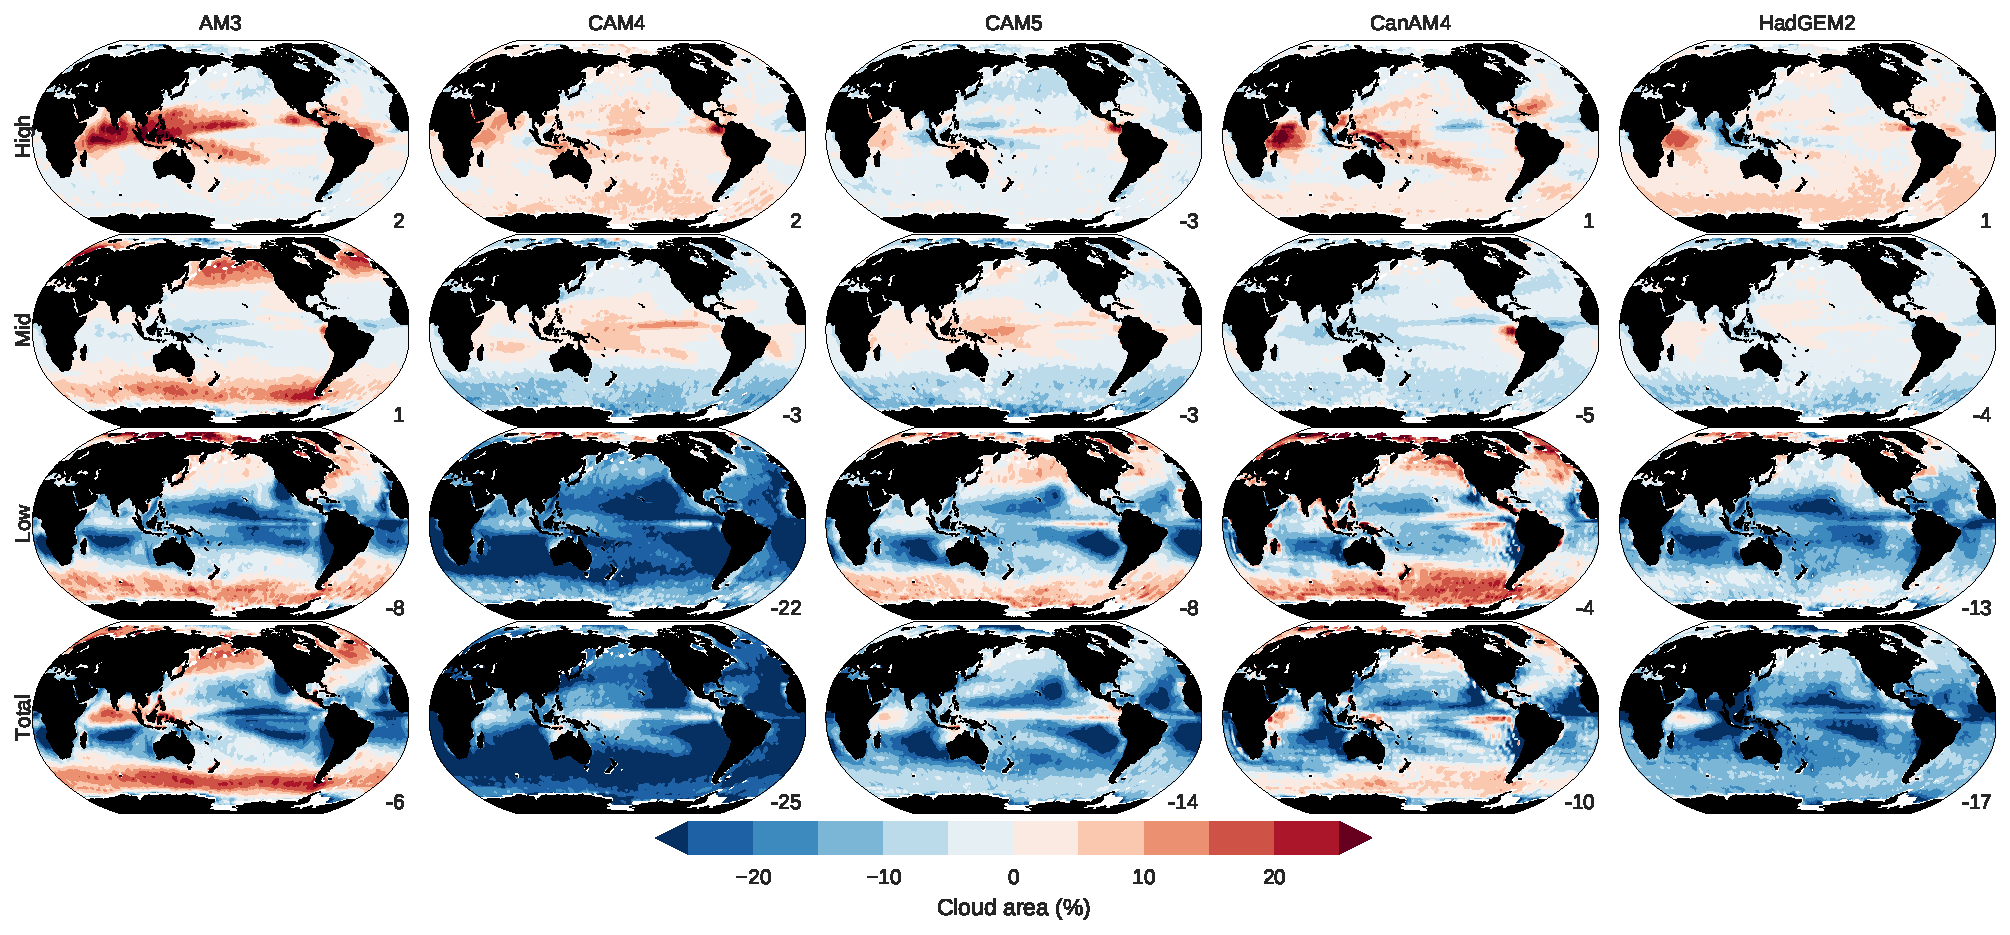
\includegraphics[width=\columnwidth]{graphics/cmip5_cldmisr_diff.pdf}
\caption{Difference in MISR-simulated total, high-topped, mid-topped, and low-topped cloud area in each of the five models relative to MISR retrievals.}
\label{cmip5_cldmisr_maps_diff}
\end{figure}

\begin{figure}
\centering
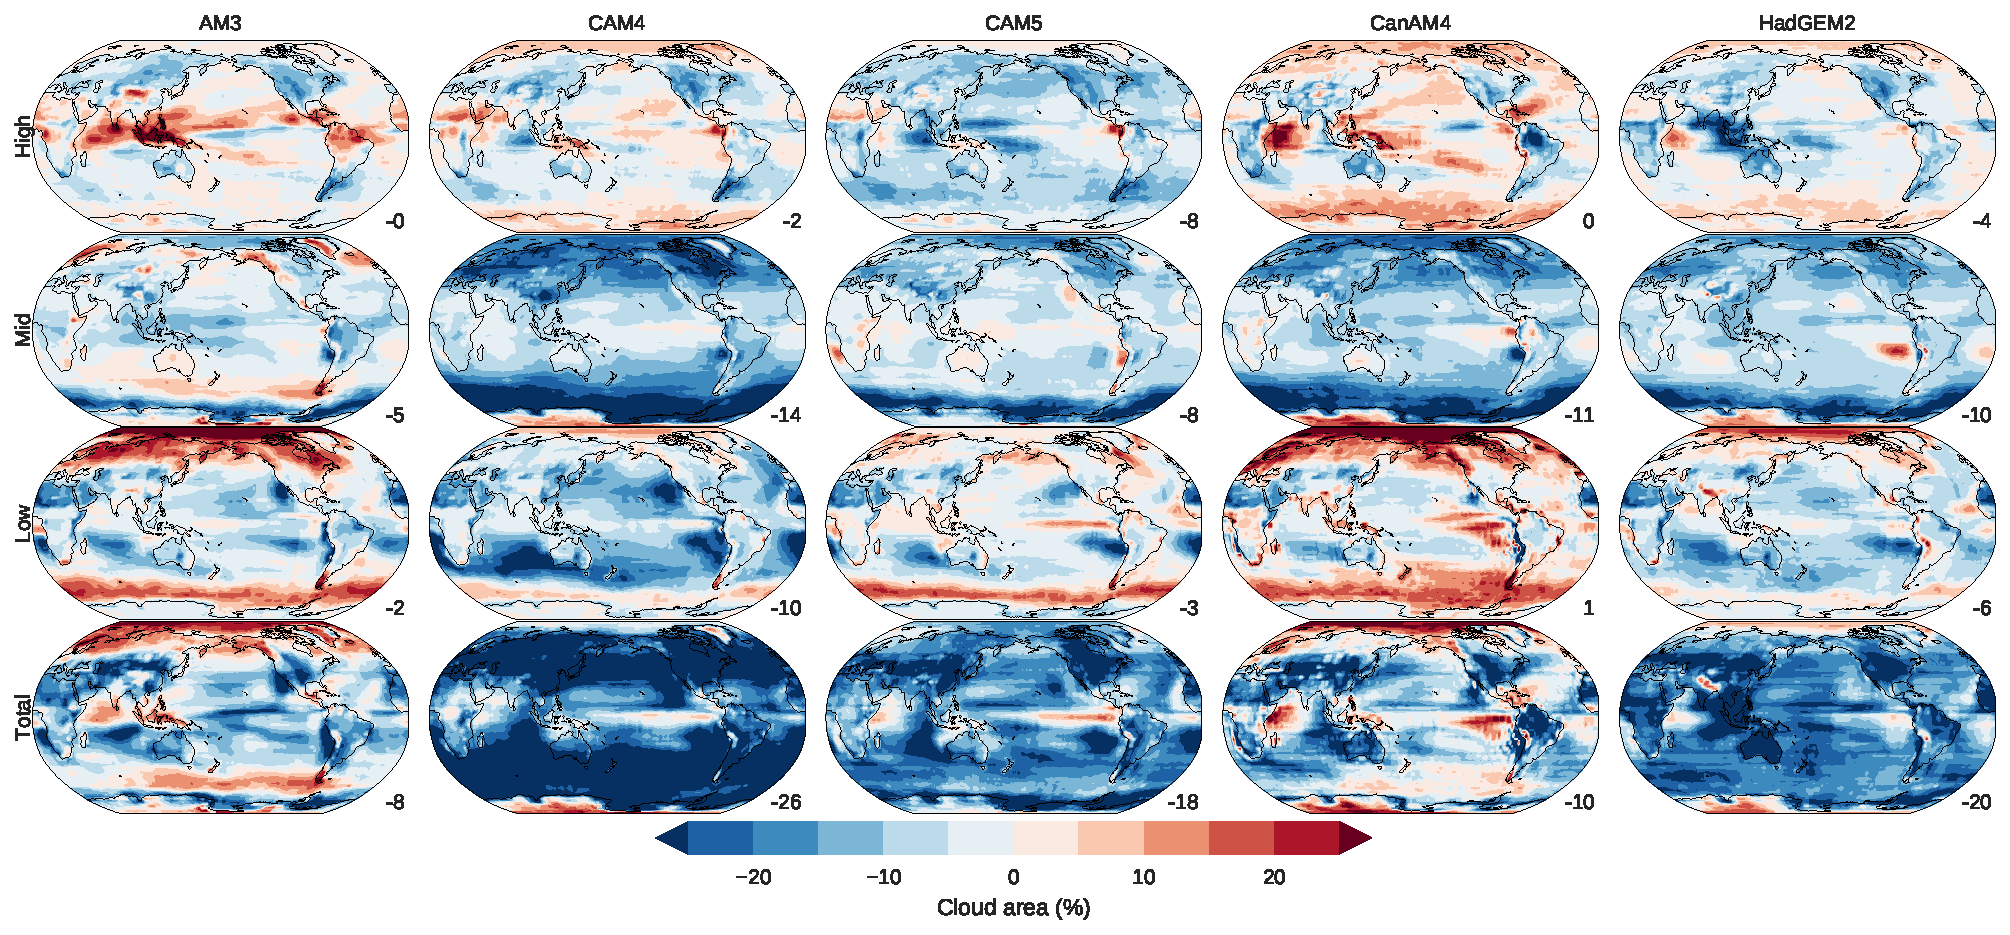
\includegraphics[width=\columnwidth]{graphics/cmip5_cldisccp_diff.pdf}
\caption{Difference in ISCCP-simulated total, high-topped, mid-topped, and low-topped cloud area in each of the five models relative to ISCCP retrievals.}
\label{cmip5_cldisccp_maps_diff}
\end{figure}


Figure \ref{cmip5_cre_maps} shows shortwave and longwave cloud radiative effects from CERES-EBAF and from each of the five models, and Figure \ref{cmip5_cre_maps_diff} shows the differences between each of the models and the CERES-EBAF observations. Indicated in each panel of each figure are the global mean values. The global means agree well between the CERES-EBAF observations and the models, with global mean differences less than 5 W/m$^2$ in all of the models. The patterns of CRE are also similar in each of the models and the observations, consistent with the well-known cloud regimes dominating different regions of the globe. The differnce plots in Figure \ref{cmip5_cre_maps_diff} show patterns of relative high differences though throughout different regions. [comments on differences specific to models...lw vs sw]. These differences are shown below to be traceable (using the simulator framework) to biases in the simulated cloud statistics.

\begin{figure}
\centering
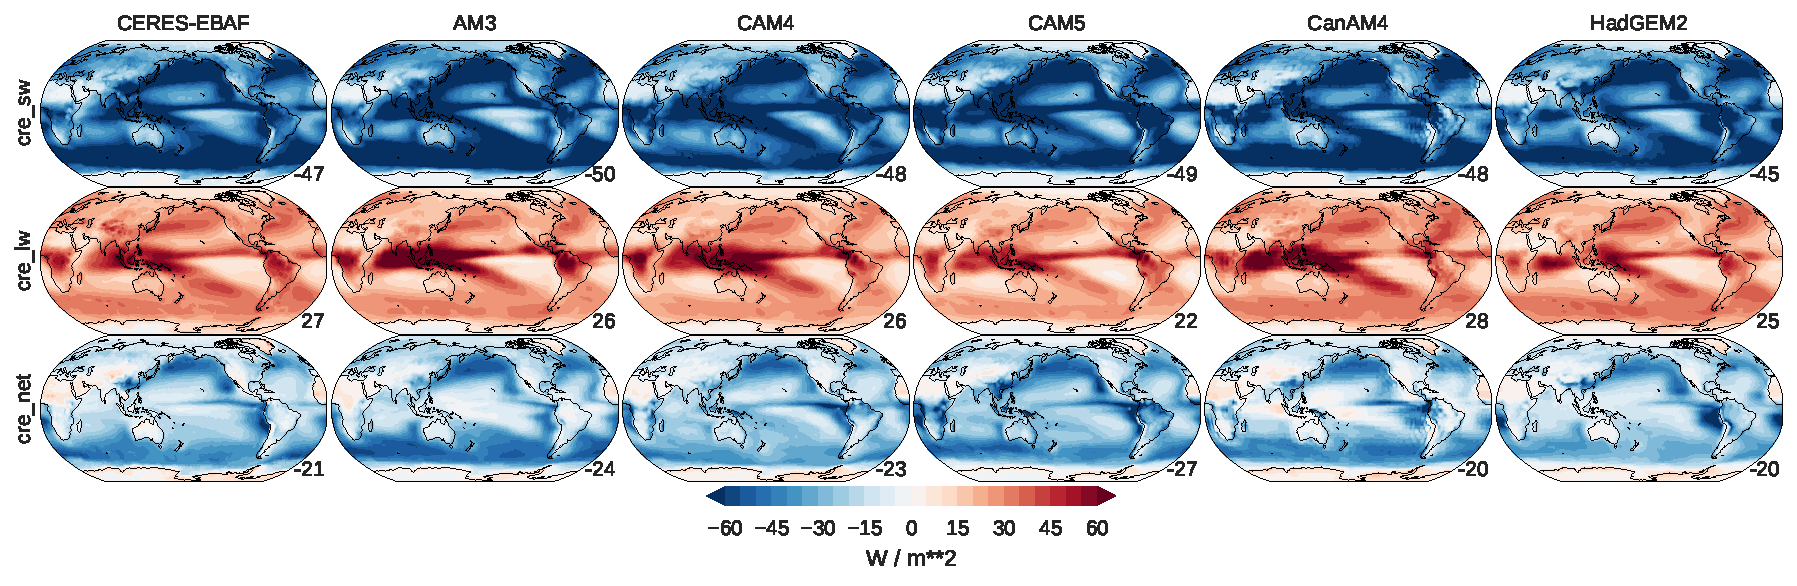
\includegraphics[width=\columnwidth]{graphics/cmip5_cre_maps.pdf}
\caption{Shortwave (top), longwave (middle) and net (bottom) cloud radiative effects from CERES-EBAF (left) and from each of the five models evaluated in this study (from left to right, AM3, CAM4, CAM5, CanAM4, HadGEM2). Numbers in the lower right corner of each map indicate the area-weighted global mean.}
\label{cmip5_cre_maps}
\end{figure}

\begin{figure}
\centering
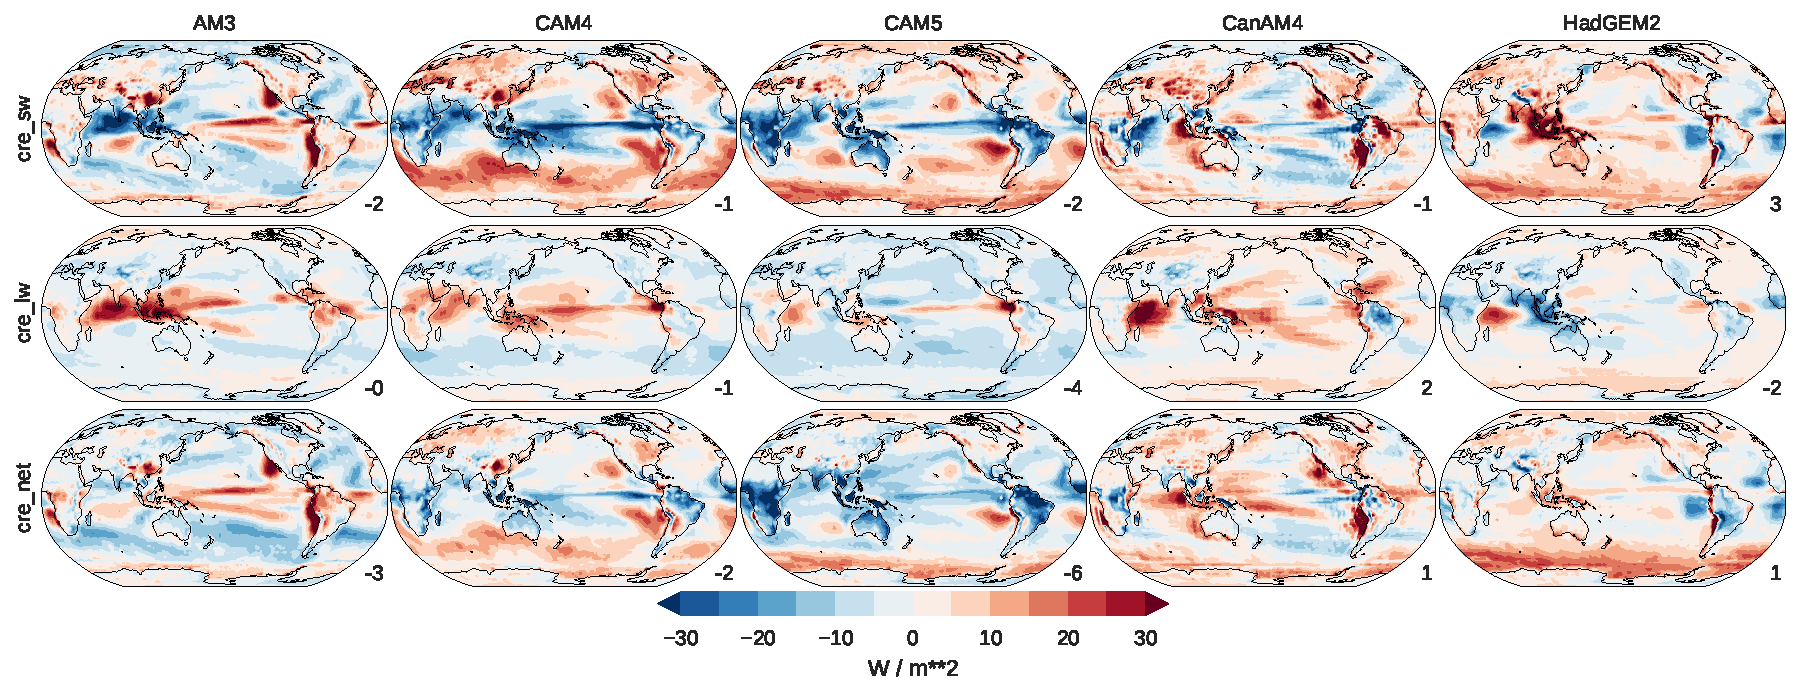
\includegraphics[width=\columnwidth]{graphics/cmip5_cre_maps_diff.pdf}
\caption{Differences in shortwave (top), longwave (middle) and net (bottom) cloud radiative effects in each of the five models relative to CERES-EBAF, calculated as model minus observations. Numbers in the lower right corner of each map indicate the area-weighted global mean of the difference.}
\label{cmip5_cre_maps_diff}
\end{figure}

Figure \ref{cmip5_cldmisr_maps_diff} and \ref{cmip5_cldisccp_maps_diff} show the differences between MISR and ISCCP-simulated total, high-topped, mid-topped, and low-topped cloud area in each of the models relative to the MISR and ISCCP retrievals. These figures highlight differences in the simulated clouds that are consistent with the differences in cloud radiative effects identified in Figure \ref{cmip5_cre_maps_diff}. [comment on specific differences...what are the magnititudes? How do these compare with the observational uncertainties idendified in Chapter \ref{misr_chapter} and the expected errors identified in Chapter \ref{subgrid1_chapter}? Also, calculate some kind of correlation between the cloud area biases and the longwave and shortwave cloud radiative effects...differences tied to radiative effects? I expect the errors to be correlated, and it would be a nice result to quantify this...]

\begin{figure}
\centering
\includegraphics[width=\columnwidth]{graphics/cmip5_clMISR_TropicalWarmPool.pdf}
\caption{Joint histograms of MISR-retrieved and MISR-simulated cloud top height and cloud optical depth for the Tropical Warm Pool.}
\label{cmip5_clMISR_TropicalWarmPool}
\end{figure}

\begin{figure}
\centering
\includegraphics[width=\columnwidth]{graphics/cmip5_clMISR_SouthernOcean.pdf}
\caption{Joint histograms of MISR-retrieved and MISR-simulated cloud top height and cloud optical depth for the Southern Ocean.}
\label{cmip5_clMISR_SouthernOcean}
\end{figure}

\section{Summary, discussion, and future directions}
This is the summary and discussion.
%% END OF CHAPTER
